\scanpage{106}
\begin{tabular}{cc}
\figure{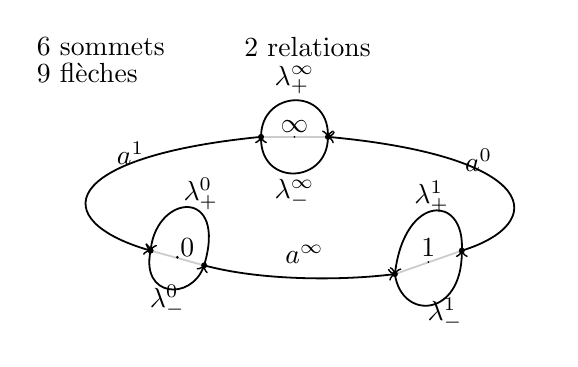
\begin{tikzpicture}[x=.85cm,y=.85cm,line width=.65pt]
\node[anchor=west] at (-.7,4.25) {6 sommets};
\node[anchor=west] at (-.7,3.85) {9 flèches};
\node[anchor=west] at (2.4,4.25) {2 relations};
\draw[gray!40] (2.8,2.9)--(3.8,2.9);
\draw[gray!40] (1.15,1.2)--(1.95,.98);
\draw[gray!40] (4.8,.85)--(5.8,1.2);
\draw[->] (2.8,2.9) .. controls (2.8,3.6) and (3.8,3.65) .. (3.8,2.9);
\draw[->] (3.8,2.9) .. controls (3.8,2.2) and (2.8,2.15) .. (2.8,2.9);
\node at (3.3,3.75) {$\lambda^\infty_+$};
\node at (3.3,2.05) {$\lambda^\infty_-$};
\fill (3.3,2.9) circle (.015); \node at (3.3,3.05) {$\infty$};
\draw[->] (1.95,.98) .. controls (2.3,2.15) and (1.25,2.05) .. (1.15,1.2);
\draw[->] (1.15,1.2) .. controls (1,.5) and (1.75,.45) .. (1.95,.98);
\node at (1.9,2.05) {$\lambda^0_+$}; \node at (1.4,.45) {$\lambda^0_-$};
\fill (1.55,1.1) circle (.022); \node at (1.7,1.25) {$0$};
\draw[->] (5.8,1.2) .. controls (5.85,2.05) and (4.95,2.05) .. (4.8,.85);
\draw[->] (4.8,.85) .. controls (4.9,.15) and (5.8,.2) .. (5.8,1.2);
\node at (5.35,2.0) {$\lambda^1_+$}; \node at (5.55,.25) {$\lambda^1_-$};
\fill (5.3,1.03) circle (.015); \node at (5.3,1.25) {$1$};
\draw[->] (2.8,2.9) .. controls (-.25,2.6) and (-.4,1.65) .. (1.15,1.2);
\node at (.85,2.65) {$a^1$};
\draw[->] (5.8,1.2) .. controls (7.1,1.6) and (7.0,2.6) .. (3.8,2.9);
\node at (6.05,2.55) {$a^0$};
\draw[->] (1.95,.98) .. controls (2.8,.75) and (4,.75) .. (4.8,.85);
\node at (3.45,1.15) {$a^\infty$};
\foreach \x/\y in {2.8/2.9,3.8/2.9,1.15/1.2,1.95/.98,4.8/.85,5.8/1.2} \fill (\x,\y) circle (.045);
\end{tikzpicture}}
&
\figure{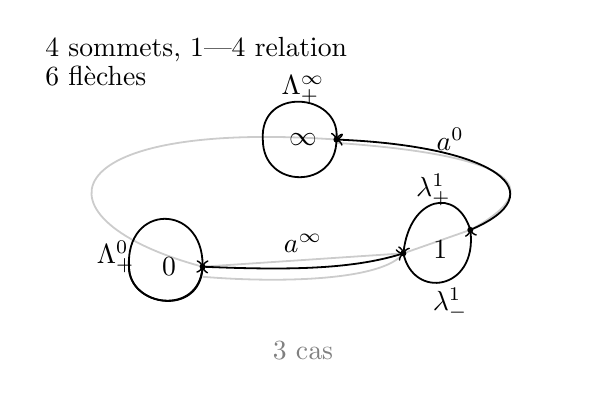
\begin{tikzpicture}[x=.85cm,y=.85cm,line width=.65pt]
\node[anchor=west] at (-.7,4.25) {4 sommets, \unsure{1|4} relation};
\node[anchor=west] at (-.7,3.85) {6 flèches};
\draw[gray!40] (3.8,2.9) .. controls (-.5,3.2) and (-.8,1.7) .. (1.8,1.0);
\draw[gray!40] (1.8,1.0)--(4.8,1.2);
\draw[gray!40] (4.8,1.2)--(5.8,1.55);
\draw[gray!40] (1.8,.85) .. controls (3,.75) and (4.5,.8) .. (4.8,1.2);
\draw[gray!40] (5.8,1.55) .. controls (7.2,2.3) and (6,2.7) .. (3.8,2.85);
\draw[->] (3.8,2.9) .. controls (3.8,2.15) and (2.7,2.15) .. (2.7,2.9) .. controls (2.65,3.7) and (3.85,3.6) .. (3.8,2.9);
\node at (3.3,3.65) {$\Lambda^\infty_+$}; \node at (3.3,2.9) {$\infty$};
\draw[->] (1.8,1.0) .. controls (1.75,.25) and (.7,.4) .. (.7,1.0) .. controls (.65,1.95) and (1.8,1.95) .. (1.8,1.0);
\draw[->] (.7,1.0) .. controls (.7,.4) and (1.75,.25) .. (1.8,1.0);
\node at (.5,1.15) {$\Lambda^0_+$}; \node at (1.3,1.0) {$0$};
\draw[->] (1.8,1.0) .. controls (3.0,.95) and (4,.95) .. (4.8,1.2);
\node at (3.3,1.35) {$a^\infty$};
\draw[->] (5.8,1.55) .. controls (5.6,2.2) and (4.9,2.05) .. (4.8,1.2);
\draw[->] (4.8,1.2) .. controls (4.95,.5) and (5.9,.65) .. (5.8,1.55);
\node at (5.25,2.15) {$\lambda^1_+$}; \node at (5.5,.45) {$\lambda^1_-$}; \node at (5.35,1.25) {$1$};
\draw[->] (5.8,1.55) .. controls (7.1,2.1) and (6.2,2.8) .. (3.8,2.9);
\node at (5.5,2.9) {$a^0$};
\foreach \x/\y in {3.8/2.9,1.8/1,4.8/1.2,5.8/1.55} \fill (\x,\y) circle (.045);
\node[gray] at (3.3,-.25) {3 cas};
\end{tikzpicture}}
\\
\figure{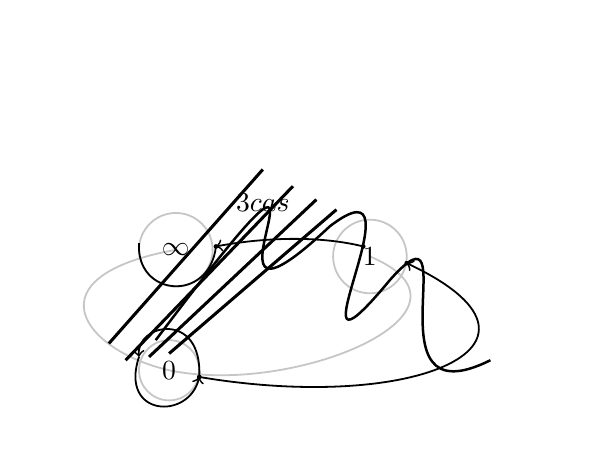
\begin{tikzpicture}[x=.85cm,y=.85cm,line width=.65pt]
\draw[gray!45] (1.2,2.7) circle (.55);
\draw[gray!45] (4.1,2.6) circle (.55);
\draw[gray!45] (1.1,.9) circle (.45);
\draw[gray!45] (1.2,2.7) .. controls (-1,2.3) and (-.2,1.2) .. (1.1,.9) .. controls (3,.5) and (6,1.8) .. (4.1,2.6);
\node at (1.2,2.7) {$\deleted{\infty}$}; \node at (4.1,2.6) {$\deleted{1}$}; \node at (1.1,.9) {$\deleted{0}$};
\draw[->] (4.0,2.75) .. controls (3.4,2.9) and (2.6,2.9) .. (1.8,2.75);
\draw (1.8,2.75) .. controls (1.7,1.9) and (.6,2.0) .. (.65,2.8);
\draw[->] (1.55,.8) .. controls (4.8,.25) and (7.2,1.3) .. (4.65,2.5);
\draw[->] (1.55,.8) .. controls (1.6,1.8) and (.6,1.6) .. (.65,1.1);
\draw[->] (.65,1.1) .. controls (.35,.2) and (1.4,.15) .. (1.55,.8);
\node at (2.5,3.4) {$\deleted{\unsure{3\text{ cas}}}$};
\foreach \x/\y in {1.8/2.75,4/2.75,4.65/2.5,1.55/.8} \fill (\x,\y) circle (.035);
\draw[line width=1.1pt] (.2,1.3)--(2.5,3.9) (.45,1.05)--(2.95,3.65) (.8,1.1)--(3.3,3.45) (1.1,1.15)--(3.6,3.3);
\draw[line width=.9pt] (.9,1.35) .. controls (4.4,6) and (1.0,.7) .. (3.5,3.05) .. controls (5.0,4.2) and (2.7,.2) .. (4.4,2.25) .. controls (5.6,3.6) and (4.0,.1) .. (5.9,1.05);
\end{tikzpicture}}
&
\figure{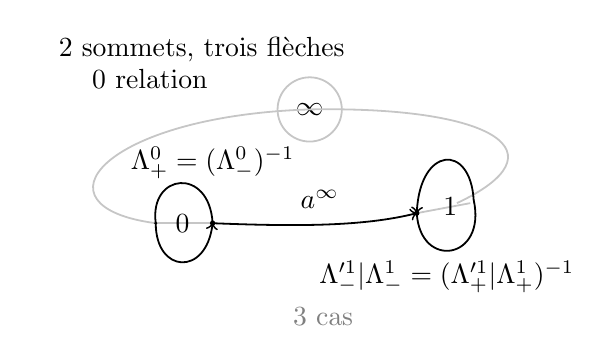
\begin{tikzpicture}[x=.85cm,y=.85cm,line width=.65pt]
\node[anchor=west] at (-.7,3.65) {2 sommets, trois flèches};
\node[anchor=west] at (-.2,3.2) {0 relation};
\draw[gray!45] (3.2,2.75) circle (.48); \node at (3.2,2.75) {$\infty$};
\draw[gray!45] (.9,1.05) .. controls (-1,1.3) and (.1,2.65) .. (3.2,2.75) .. controls (6.0,2.8) and (7.0,2.1) .. (5.4,1.35);
\draw[gray!45] (.9,1.05)--(1.75,1.05); \draw[gray!45] (4.8,1.2)--(5.6,1.35);
\draw[->] (1.75,1.05) .. controls (1.7,1.9) and (.8,1.8) .. (.9,1.05) .. controls (.9,.3) and (1.65,.25) .. (1.75,1.05);
\fill (.9,1.05) circle (.025); \fill (1.75,1.05) circle (.04); \node at (1.3,1.05) {$0$};
\node at (1.75,1.95) {$\Lambda^0_+=(\Lambda^0_-)^{-1}$};
\draw[->] (1.75,1.05) .. controls (3,1.0) and (4,1.0) .. (4.8,1.2);
\node at (3.35,1.4) {$a^\infty$};
\draw[->] (4.8,1.2) .. controls (4.85,.35) and (5.85,.5) .. (5.65,1.4) .. controls (5.6,2.25) and (4.85,2.2) .. (4.8,1.2);
\fill (4.8,1.2) circle (.04); \node at (5.3,1.3) {$1$};
\node at (5.25,.25) {$\unsure{\Lambda^{\prime1}_-|\Lambda^1_-}=(\unsure{\Lambda^{\prime1}_+|\Lambda^1_+})^{-1}$};
\node[gray] at (3.4,-.35) {3 cas};
\end{tikzpicture}}
\\
\figure{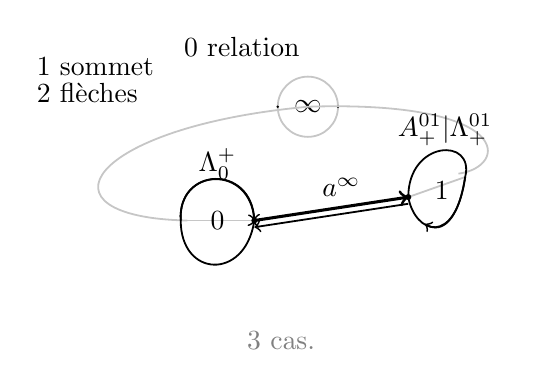
\begin{tikzpicture}[x=.85cm,y=.85cm,line width=.65pt]
\node[anchor=west] at (-.7,3.5) {1 sommet};
\node[anchor=west] at (-.7,3.1) {2 flèches};
\node[anchor=west] at (1.5,3.8) {0 relation};
\draw[gray!45] (3.5,2.9) circle (.45); \node at (3.5,2.9) {$\infty$};
\fill (3.05,2.9) circle (.022); \fill (3.95,2.9) circle (.022);
\draw[gray!45] (1.7,1.2) .. controls (-.65,1.25) and (.2,2.6) .. (3.5,2.9) .. controls (6.6,3) and (6.5,2.0) .. (5.75,1.9);
\draw[gray!45] (1.6,1.2)--(2.7,1.2); \draw[gray!45] (5,1.55)--(5.85,1.85);
\draw[->] (2.7,1.2) .. controls (2.65,2.05) and (1.55,2.0) .. (1.6,1.2) .. controls (1.6,.35) and (2.55,.3) .. (2.7,1.2);
\draw[->] (1.6,1.2) .. controls (1.55,2.0) and (2.65,2.05) .. (2.7,1.2);
\node at (2.15,2.05) {$\Lambda_0^+$}; \node at (2.15,1.2) {$0$};
\draw[->,line width=1.1pt] (2.7,1.2)--(5,1.55);
\draw[->] (5,1.45)--(2.7,1.1);
\node at (4,1.7) {$\deleted{\unsure{a^\infty}}$};
\draw (5,1.55) .. controls (5,2.4) and (6,2.45) .. (5.85,1.85) .. controls (5.7,.8) and (5.1,1.0) .. (5,1.55);
\draw[->] (5.85,1.85) .. controls (5.75,1.2) and (5.5,1.0) .. (5.25,1.15);
\node at (5.55,2.55) {$\unsure{A_+^{01}|\Lambda_+^{01}}$}; \node at (5.5,1.65) {$1$};
\fill (2.7,1.2) circle (.045); \fill (5,1.55) circle (.045);
\node[gray] at (3.1,-.6) {3 cas.};
\end{tikzpicture}}
&
\end{tabular}
\mspage{105}
